%\documentclass[jou]{apa6}
\documentclass[11pt]{article}
\usepackage{ucs}
\usepackage[utf8x]{inputenc}
\usepackage{changepage}
\usepackage{graphicx}
\usepackage{amsmath}
\usepackage{gensymb}
\usepackage{amssymb}
\usepackage{enumerate}
\usepackage{tabularx}
\usepackage{lipsum}
\usepackage{hyperref}
\usepackage{fancyvrb}

\oddsidemargin 0.0in
\evensidemargin 0.0in
\textwidth 6.27in
\headheight 1.0in
\topmargin -0.1in
\headheight 0.0in
\headsep 0.0in
\textheight 9.0in

\usepackage{xcolor}

\setlength\parindent{0pt}

\newenvironment{myenv}{\begin{adjustwidth}{0.4in}{0.4in}}{\end{adjustwidth}}
\renewcommand{\abstractname}{Anotācija}
\renewcommand\refname{Atsauces}



\newcounter{alphnum}
\newenvironment{alphlist}{\begin{list}{(\Alph{alphnum})}{\usecounter{alphnum}\setlength{\leftmargin}{2.5em}} \rm}{\end{list}}


%16.3-6

\makeatletter
\let\saved@bibitem\@bibitem
\makeatother

\usepackage{bibentry}
%\usepackage{hyperref}


%\title{Homework 1: Grading Criteria}
%\author{Kalvis}
%\affiliation{RBS}



\begin{document}
\thispagestyle{empty}

%\twocolumn


\begin{center}
{\Large Sample Assignment 1, 2020-09-09}
\end{center}




{\bf Question 1 (Bitwise Operations).} Write the output
(and the content of variables {\tt a,b,c} in hexadecimal notation),
after this snipped is executed:
\begin{Verbatim}[frame=single]
int a = 47;
int b = -13;
char c = 'c';
cout << (a & b) << endl;  // bitwise AND
cout << (a | b) << endl;  // bitwise OR
cout << (~b) << endl;     // bitwise NOT
\end{Verbatim}



\vspace{10pt}
{\bf Question 2 (Compilation and Linking).} 

All these command-lines are frequently used to deal with 
C++ code on Linux. Match the commands with their informal 
descriptions. 

\begin{verbatim}
(1)  g++ -Wall -g -o Hello Hello.cpp
(2)  g++ -o Hello Hello.cpp; chmod a+x Hello; ./Hello
(3)  g++ -o Myprogram Myprogram.o MyprogramMain.o
(4)  g++ -o Myprogram.o -c Myprogram.cpp
(5)  ./Hello >> out.txt
\end{verbatim}

\begin{enumerate}[(A)]
\item Compile and link a C++ program, then run it.
\item Run a program, append its STDOUT (cout) to file {\tt out.txt}
\item Just compile a program into an object file.
\item Compile and link a C++ program, include warnings and debug info.
\item Just link a program from object files.
\end{enumerate}



%% https://www3.ntu.edu.sg/home/ehchua/programming/cpp/gcc_make.html

{\bf Question 3 (Makefiles).} 

Draw the "make" evaluation tree, if the user types {\tt make all}\\
At the top of this tree specify the target {\tt all}, 
then draw all all its prerequisites as children, 
then draw their children, if any, etc. Do this until you reach targets 
without any prerequisites.

Describe in English, what values are contained in 
{\tt SRCFILES} and {\tt OBJFILES}.


\begin{Verbatim}[frame=single]
SRCFILES := $(wildcard ./*.cpp)
OBJFILES := $(patsubst ./%.cpp,./%.o,$(SRCFILES))

clean:
	rm -f hello.o hello.exe *out.txt

all: hello.exe

hello.exe: hello.o hellomain.o
	g++ -o hello.exe hello.o hellomain.o

hello.o: hello.cpp
	g++ -c hello.cpp

hellomain.o: hellomain.cpp
	g++ -c hellomain.cpp
\end{Verbatim}


{\bf Question 4 (for loops).}

Consider a regular "for" loop like this: 
\begin{verbatim}
for (int i =0; i<100; i++) { /* ... */ }
\end{verbatim}

\begin{enumerate}
\item Is it legal to change the loop variable {\tt i} 
in the body of the loop?
\item Is it legal to use the value {\tt i} after the loop 
has finished?
\item Can we omit the any of the three parts in the {\tt for}-loop?
Can we omit all $3$ parts as in this loop: {\tt for (;;) { /* ... */ }}
\end{enumerate}



\vspace{5mm}
\begin{tabular}{@{}ll@{}} 
\begin{minipage}{0.48\columnwidth}
{\bf Question 5 (Flowchart).} 
Write C++ code with branch and loop statements
(possibly, including "break" and "continue") to 
implement the flowchart shown in the picture.
\end{minipage} &
\begin{minipage}{0.5\columnwidth}
\begin{center}
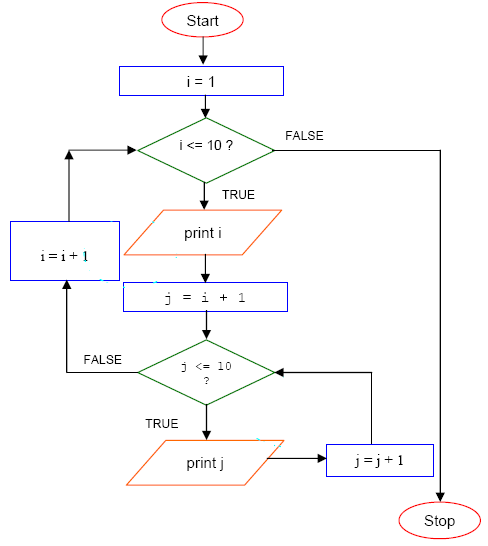
\includegraphics[width=3in]{sample-assignment01-flowchart.png}
\end{center}
\end{minipage}
\end{tabular}


{\bf Question 6 (do-while loops).}

For the code snippet below draw an equivalent flowchart. 
Does the "continue" statement jump to the bottom 
of the do-while loop (and retests the condition); 
or does it jump to the top of the do-while loop?
If you pass "null" user to the method {\tt isLast()} 
the program might crash.

\begin{Verbatim}[frame=single]
User user = userDao.GetNext();
do {
    // process some user
    user = userDao.GetNext(user.Id);
    if (user == null) { continue; }
    // do more procesing for the user. 
}
while (!user.isLast())
\end{Verbatim}






\end{document}



